% !TEX root = Master.tex

While the previously described data will be used for modelling, data captured by the airborne LiDAR is of main interested in this report, since the ability of innovating forest inventory is discussed.\\

LiDAR uses a laser scanning system to capture distances. In context, laser scanning is referred to the active emitting and sensing of light. Thus, Light Detection and Ranging is a suitable description of the mechanics, also known as LADAR (Laser Detection and Ranging). LiDAR is a more generalized definition, as instead of laser- light also xenon or flash lamps can be used [2]. A high-level definition of the functionality of LiDAR is as follows. Laser beams are continuously emitted of the LiDAR system, mounted on an airborne vehicle. The coordinates are throughout captured by a GPS (Global Positioning System) and IMU (Inertial Measurement Unit – used to capture adjust for e.g. inclined positioning, acceleration of the vehicle). Laser or xeon/flash light is emitted of an active sensor and the distance captured once it is traveled back to the scanner. As forests have a relatively turbulent surface and only little light can reach the surface of the forest, many systems only capture the first and last impulse [3]. The cloud of captured points can then be used to create a 3-D image of the forest (see Figure \ref{fig:LiDAR}).

\begin{figure}[H]
  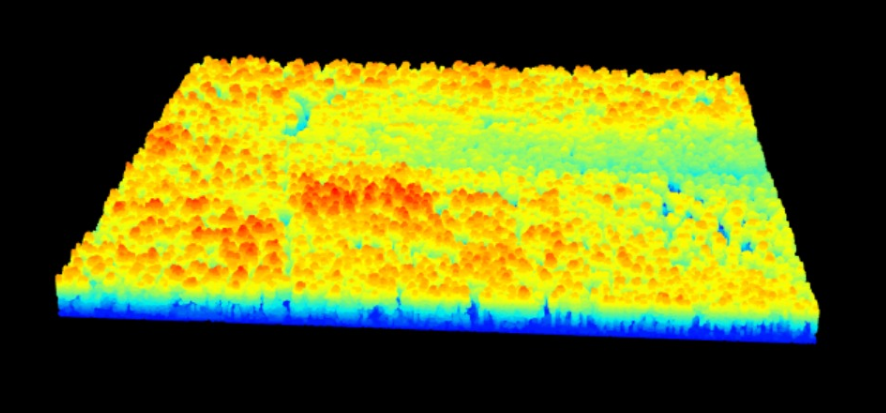
\includegraphics[width=\textwidth]{lidar.png}
  \caption{3-D Image of a small area of the forest of Gartow made by the airborne LiDAR. The determined height is colorized. A
dense group of height trees is found almost in the middle and directly behind an aisle of small trees.}
  \label{fig:LiDAR}
\end{figure}

Main benefits of LiDAR compared to other systems is the ability to capture data regardless of sun positioning, day or night and the ability to map through the highly dense areas (the canopies of the trees). The main benefit compared to the traditional way of forest inventory is relative intuitive. A plane is capable of objectively measuring the forest subject to this report in under a week; while a forester must inspect every single hectare, providing a more subjective intuition of the forest inventory.

\begin{table}[H]
\setlength\arrayrulewidth{1pt}  
\centering
\begin{adjustbox}{max width=\textwidth}
\begin{tabular}{|c|c|}
\hline
\rowcolor{Gray}
\textbf{Flight Altitude}              & \textbf{Approx. 590m above ground} \\ \hline
Nominal point density (laser)         & 6 points / m²                      \\ \hline
Ground resolution                     & 4.3cm                              \\ \hline
Point density (to circumvent overlap) & 12 points / m²                     \\ \hline
Ground resolution                     & 4.3cm                              \\ \hline
\end{tabular}
\end{adjustbox}
\caption{Flight log of the airborne laser scanning of the forest of Gartow [12]}
\label{tab:Flight log}
\end{table}

ForestEye Research GmbH \& Co. KG provided the detected single tree location, tree species and canopy area based on LiDAR.